\section{Results}
In this simulation experiment, we consider a team of $N = 6$ robots with radius $r_R = 0.15$m and maximum pushing force $f_{\max} = 10$N, which cooperatively perform an estimation task to obtain the CoM of a U-shaped object. The object has a mass of $m = 3$kg and a moment of inertia $I = 0.1$kg$\cdot$m$^2$. First, the formation synthesis problem is addressed using ALPSO to determine the optimal robot configuration. The obtained formation is illustrated in Fig.~\ref{fig:formation}.
After the robots move to their designated positions, each robot independently solves the quadratic programming problem to determine its pushing force while maintaining zero resultant force and generating a torque close to the desired value $\tau_d$. The resulting pushing forces are also annotated in Fig.~\ref{fig:formation}. The vertical forces of robots R2 and R5 ($3.8$\,N each) and the horizontal forces of robots R4 and R6 ($2.8$\,N each) cancel out pairwise, yielding zero net force, while the offset between the lines of action of each pair generates the desired torque. Robots R1 and R3 exert no force, indicating that the desired torque can be achieved without them; nevertheless, they remain in contact with the object and still contribute to the estimation.

\begin{figure}[htbp]
\centering
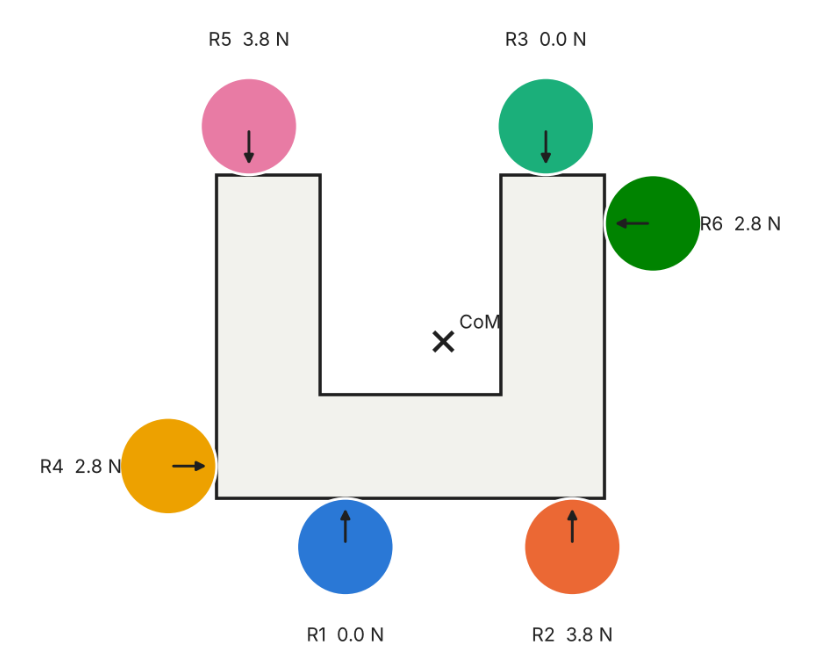
\includegraphics[width=0.6\linewidth]{Result/figures/formation.png}
\caption{Optimal formation of $N=6$ robots around the U-shaped object obtained by ALPSO, with the pushing force of each robot computed by the force control problem. The arrows indicate the force directions, and the cross marks the true CoM.}
\label{fig:formation}
\end{figure}

During the rotational motion, each robot independently estimates the object's CoM using Recursive Least Squares (RLS), based on successive measurements of its contact point position and velocity and the object's angular velocity. Note that, since the contact point is assumed to be fixed relative to the robot, its position and velocity can be derived from the robot's pose, linear velocity, and angular velocity.
To account for sensing imperfections, the contact point position and velocity and the object's angular velocity measured by each robot are corrupted by independent zero-mean Gaussian white noise with standard deviations $\sigma_p = 2$\,mm, $\sigma_v = 0.01$\,m/s and $\sigma_\omega = 0.02$\,rad/s, respectively.

\begin{figure}[H]
\centering
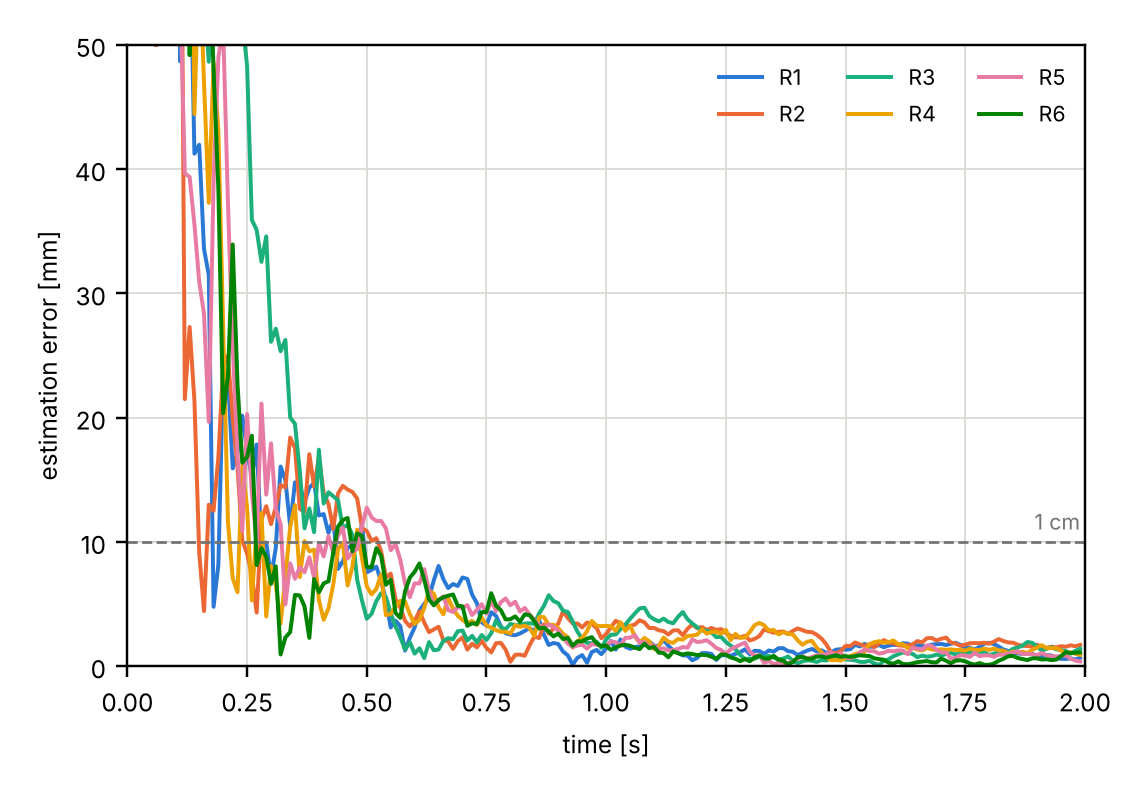
\includegraphics[width=0.75\linewidth]{Result/figures/estimation_error.png}
\caption{CoM estimation error of each robot over time. The dashed line indicates an error of $1$\,cm.}
\label{fig:estimation_error}
\end{figure}

The estimation errors of all robots are shown in Fig.~\ref{fig:estimation_error}. Large errors are observed initially, since few measurements are available and the angular velocity of the object is still small at the onset of rotation. As more measurements are collected, the estimates of all robots converge rapidly, with the errors falling below $1$\,cm within approximately $0.75$\,s. After $2$\,s, the estimation errors of all robots remain below $2$\,mm. Moreover, the estimates of the six robots converge to nearly the same value, showing that each robot can independently obtain an accurate CoM estimate without sharing its measurements.
